In this section, the layer is described in some detail in terms of its specific subsystems. Describe each of the layers and its subsystems in a separate chapter/major subsection of this document. The content of each subsystem description should be similar. Include in this section any special considerations and/or trade-offs considered for the approach you have chosen.

\subsection{MIDI decoder}
pending
\begin{figure}[h!]
	\centering
 	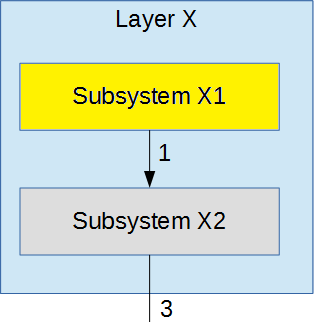
\includegraphics[width=0.60\textwidth]{images/subsystem}
 \caption{Example subsystem description diagram}
\end{figure}

\subsubsection{Assumptions}
pending

\subsubsection{Responsibilities}
pending

\subsubsection{Subsystem Interfaces}
pending

\begin {table}[H]
\caption {Subsystem interfaces} 
\begin{center}
    \begin{tabular}{ | p{1cm} | p{6cm} | p{3cm} | p{3cm} |}
    \hline
    ID & Description & Inputs & Outputs \\ \hline
    \#xx & Description of the interface/bus & \pbox{3cm}{input 1 \\ input 2} & \pbox{3cm}{output 1}  \\ \hline
    \#xx & Description of the interface/bus & \pbox{3cm}{N/A} & \pbox{3cm}{output 1}  \\ \hline
    \end{tabular}
\end{center}
\end{table}

\subsection{Speaker}
The speaker gives the final output of the laser harp. After all the processing of the data in the raspberry pi, the pi sends the final output of the sound signal to the speakers. The speakers produce the desired sound as output. 

\begin{figure}[h!]
	\centering
 	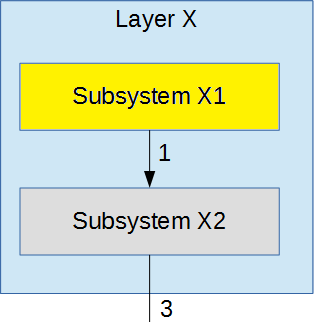
\includegraphics[width=0.60\textwidth]{images/subsystem}
 \caption{Example subsystem description diagram}
\end{figure}

\subsubsection{Assumptions}
The speaker is connected via USB A cable to the pi. It is also powered by the same battery powering the Raspberry Pi.

\subsubsection{Responsibilities}
The speaker should produce decent sound output with no interference. It should be loud enough so the sound can be heard in a conference hall. 

\subsubsection{Subsystem Interfaces}
The speaker gets analog signals from the raspberry pi and converts it into sound waves as output. This is the final output of the system. The speaker is connected via USB A cable to the system.

\begin {table}[H]
\caption {Subsystem interfaces} 
\begin{center}
    \begin{tabular}{ | p{1cm} | p{6cm} | p{3cm} | p{3cm} |}
    \hline
    ID & Description & Inputs & Outputs \\ \hline
    \#xx & Description of the interface/bus & \pbox{3cm}{input 1 \\ input 2} & \pbox{3cm}{output 1}  \\ \hline
    \#xx & Description of the interface/bus & \pbox{3cm}{N/A} & \pbox{3cm}{output 1}  \\ \hline
    \end{tabular}
\end{center}
\end{table}

\subsection{FluidSynth}
FluidSynth is a real-time software synthesizer based on the SoundFont 2 specifications and has reached widespread distribution. It converts the MIDI signals to produce desired sound waves.

\begin{figure}[h!]
	\centering
 	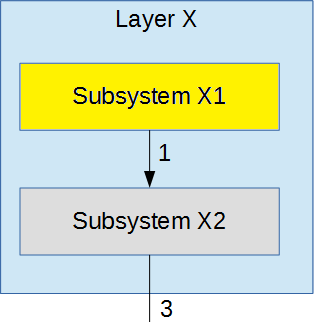
\includegraphics[width=0.60\textwidth]{images/subsystem}
 \caption{Example subsystem description diagram}
\end{figure}

\subsubsection{Assumptions}
The software already has default preset sounds built-in. It also has the functionality manipulate the sound to produce various sound effects. Also it is free, open source and easy to use.

\subsubsection{Responsibilities}
The software is used to convert MIDI signals to sound waves. It should have multiple different sound effects and create a wide range of sound octaves in different formats.

\subsubsection{Subsystem Interfaces}
The software is downloaded and installed into the raspberry pi. It is supported by the Raspian OS.

\begin {table}[H]
\caption {Subsystem interfaces} 
\begin{center}
    \begin{tabular}{ | p{1cm} | p{6cm} | p{3cm} | p{3cm} |}
    \hline
    ID & Description & Inputs & Outputs \\ \hline
    \#xx & Description of the interface/bus & \pbox{3cm}{input 1 \\ input 2} & \pbox{3cm}{output 1}  \\ \hline
    \#xx & Description of the interface/bus & \pbox{3cm}{N/A} & \pbox{3cm}{output 1}  \\ \hline
    \end{tabular}
\end{center}
\end{table}
